\documentclass[]{beamer}
\usepackage{xmpmulti}
\usepackage{psfrag}
\usepackage{color}
\usepackage{tcolorbox}

\newcommand{\owner}{\mathcal{O}}
\newcommand{\manager}{\mathcal{M}}

\mode<presentation>
{\usetheme{Boadilla}  % very plain
}

\usepackage{xcolor}

\usepackage{amssymb,amsmath,amsthm}
\usepackage{boxedminipage}

\usepackage{tikz}
\usetikzlibrary{snakes}
\usetikzlibrary{backgrounds} 
\usepackage{pgfmath}

%%MACROS
\newcommand{\Sender}{\color{teal} \mathsf{S}}
\newcommand{\Receiver}{\color{teal} \mathsf{R}}
\newcommand{\zu}{\{0,1\}}
\newcommand{\from}{\leftarrow}
\newcommand{\ds}{\mathsf{DS}}
\newcommand{\expt}{\mathsf{Expt}}
\newcommand{\calA}{\mathcal{A}}
\newcommand{\calL}{\mathcal{L}}
\newcommand{\calR}{\mathcal{R}}
\newcommand{\calS}{\mathcal{S}}
\newcommand{\mem}{\mathsf{memory}}
\newcommand{\re}{\mathsf{read}}
\newcommand{\wri}{\mathsf{write}}
\newcommand{\mr}{\mathsf{Read}}
\newcommand{\mw}{\mathsf{Write}}
\newcommand{\mrl}{\mathsf{LRead}}
\newcommand{\mwl}{\mathsf{LWrite}}
\newcommand{\bB}{\mathbf{B}}

\newcommand{\cnt}{\mathtt{cnt}}
\newcommand{\tpp}{\mathtt{top}}
\newcommand{\init}{\mathsf{Init}}
\newcommand{\push}{\mathsf{Push}}
\newcommand{\pop}{\mathsf{Pop}}
\newcommand{\enc}{\mathsf{Enc}}


\title[]{Limits of Breach-Resistant and Snapshot-Oblivious RAMs}
\subtitle{\color{teal} Still $\Omega(b/w\cdot\log (nb/c))$}

\author{\color{purple} Giuseppe Persiano}

\institute[S+G]{\color{purple} Universit\`a di Salerno and Google LLC}

\date[ESSA 3]{\color{red} ESSA 3 in Bertinoro}

\begin{document}

\newcommand{\ignore}[1]{}

\begin{frame}
  \titlepage

{\color{brown}
Joint work with Kevin Yeo (Google LLC and Columbia U.)

Accepted to CRYPTO 23
}
\end{frame}

\begin{frame}
\frametitle{RAMS}

\begin{center}
\only<1>{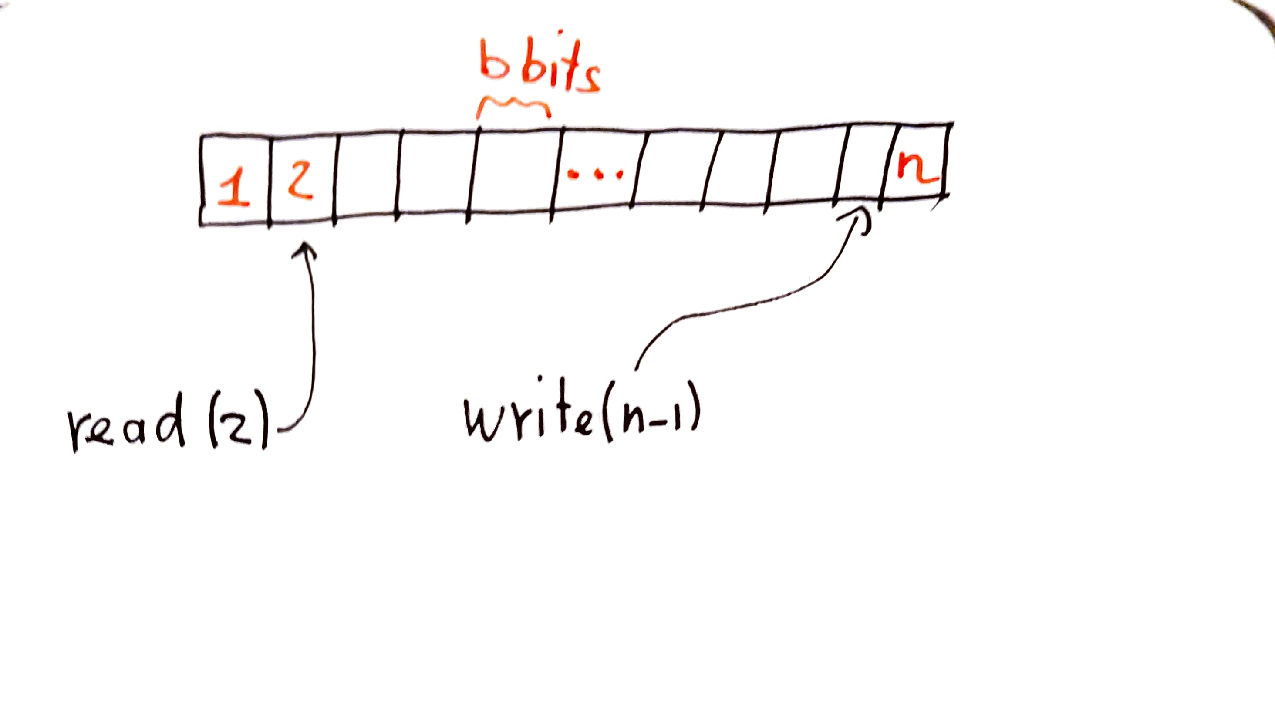
\includegraphics[width=\textwidth]{Images/RAM-01.pdf}}
\only<2->{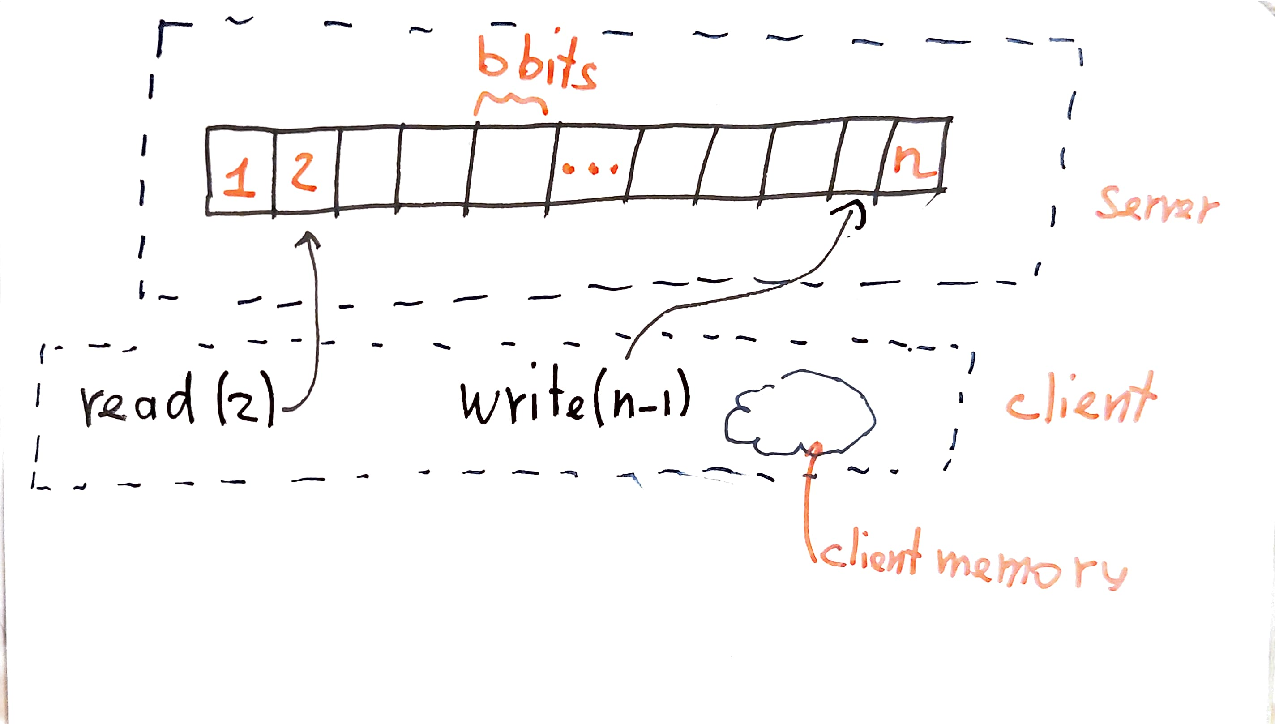
\includegraphics[width=\textwidth]{Images/RAM-02-A.pdf}}
\end{center}
\only<3>{

\color{red}

Server memory words of length $w<b$
}

\end{frame}

\begin{frame}
\frametitle{Oblivious RAMS}

Hiding the access pattern to the RAM from the server

\begin{block}{Upper bounds}
\begin{itemize}
\item Goldreich Ostrovsky -- Late 80's early 90'
    \begin{itemize}
        \item Slowdown $\color{teal}O(\log^3 n)$
    \end{itemize}
\item ....
\item Patel Persiano Raykova Yeo --  2018 
    \begin{itemize}
        \item Slowdown $\color{teal}O(\log n\log\log n)$
    \end{itemize}
\item Asharov Komogordsky Lin Peserico Shi --  2018 
    \begin{itemize}
        \item Slowdown $\color{teal}O(\log n)$
    \end{itemize}
\end{itemize}
\end{block}

\pause
\begin{block}{Lower bounds}
\begin{itemize}
\item Larsen Nielsen -- 2018
    \begin{itemize}
        \item Slowdown $\color{teal}\Omega(\log n)$
    \end{itemize}
\item It holds also for Differential Privacy, some leakage
\end{itemize}
\end{block}
\end{frame}

\begin{frame}
\frametitle{The snapshot adversary}

the {\color{blue} Server} is the adversary

\begin{block}{Snapshot Adversary}
Du, Genkin, Grubbs, 2022

\begin{itemize}
\item The adversary gets control of the {\color{blue} Server}
for $L$ {\color{red} consecutive} operations
\begin{itemize}
    \item Slowdown $\color{magenta} O(\log L)$
\end{itemize}
\end{itemize}
\end{block}

\pause

\vfill

What if the adversary is active for more than one {\em\color{blue} window}?
\end{frame}


\begin{frame}
\frametitle{Snapshot Resistant Stacks}

\begin{itemize}
\item 
\only<1>{{\color{teal} \bf read -- write}}
\only<2->{{\color{teal} \bf push -- pop}}

\only<3->{
\item \color{teal} want to hide sequence of operations
\begin{itemize}
    \item hide if {\color{teal} \bf push} or {\color{teal} \bf pop}
    \item hide input to {\color{teal} \bf push}
\end{itemize}
}

\only<4->{
    \item hiding from whom
\begin{itemize}
        \item Adversary that can see $\color{blue} S$ memory snapshots
        \item Adversary that can see $\color{blue} T$ operations transcripts
\end{itemize}
    
}
\end{itemize}
\end{frame}

\begin{frame}
\frametitle{$(\infty,0)$-snapshot secure stacks}

Adversary gets snapshots of memory after {\color{red} all operations} and {\color{red} no transcript}

\vskip .2cm

$\qquad$ $\color{blue} S=\infty$ \hfill $\color{blue} T=0$ $\qquad$

\begin{center}
\only<1>{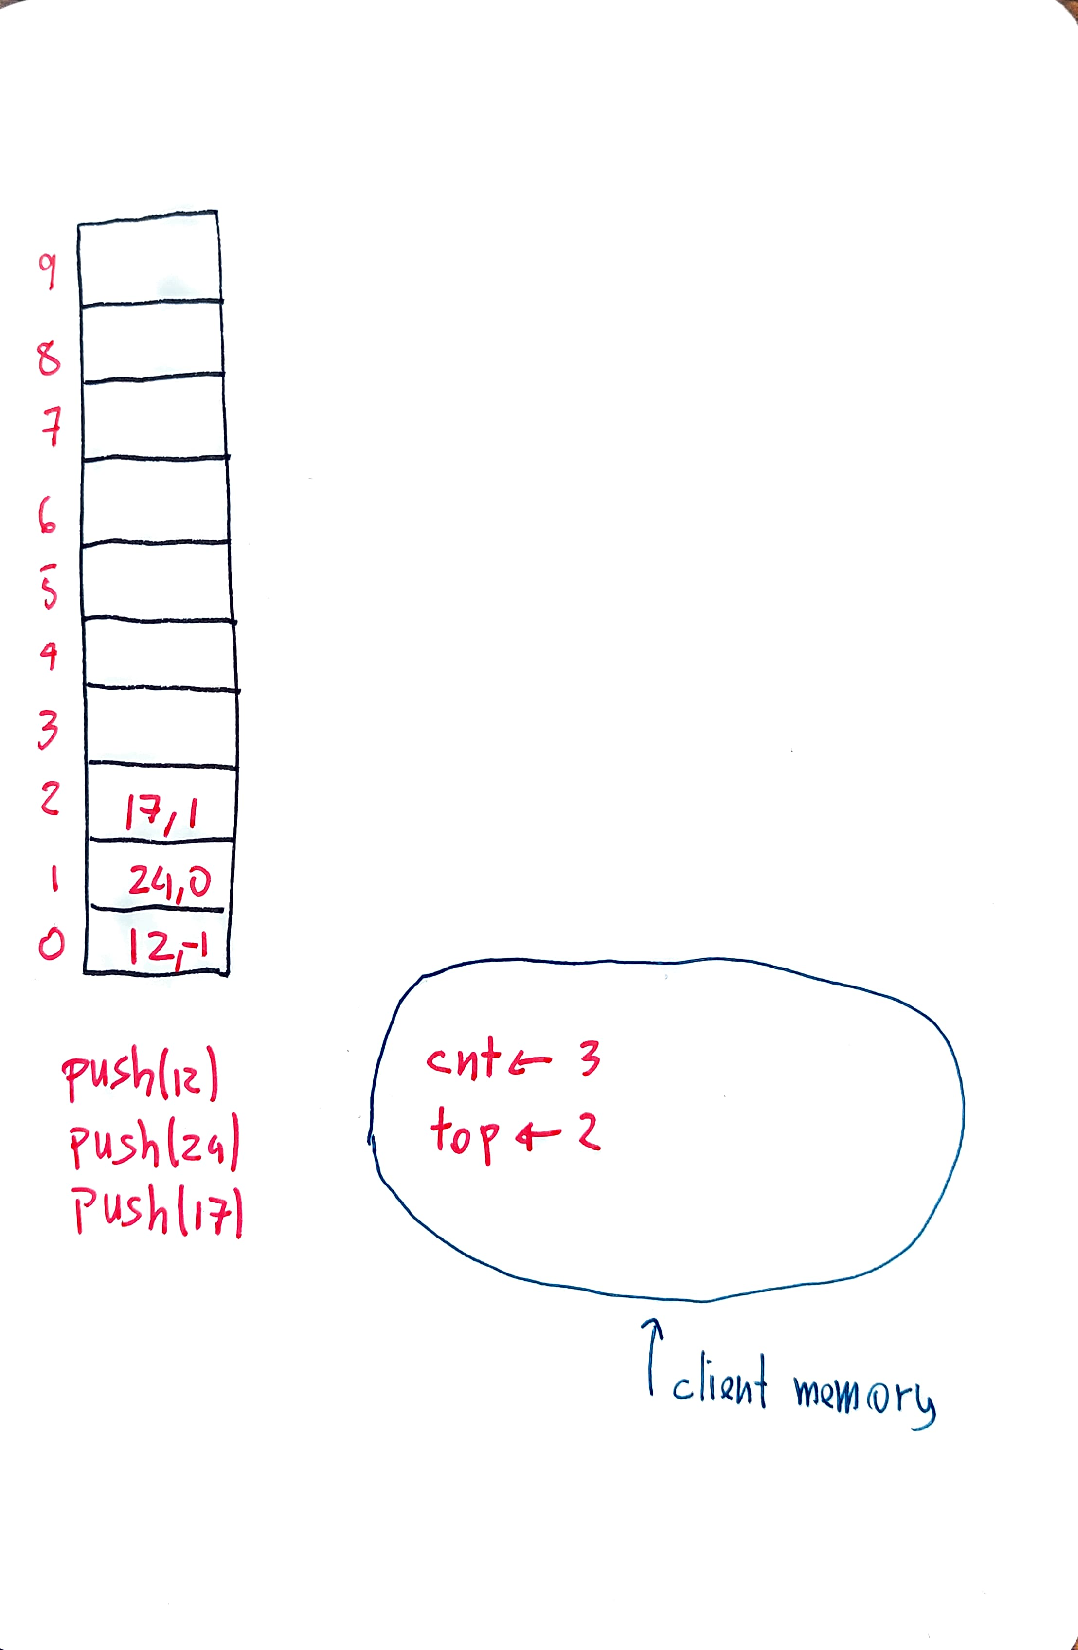
\includegraphics[height=9cm]{Images/stack-01.pdf}}
\only<2>{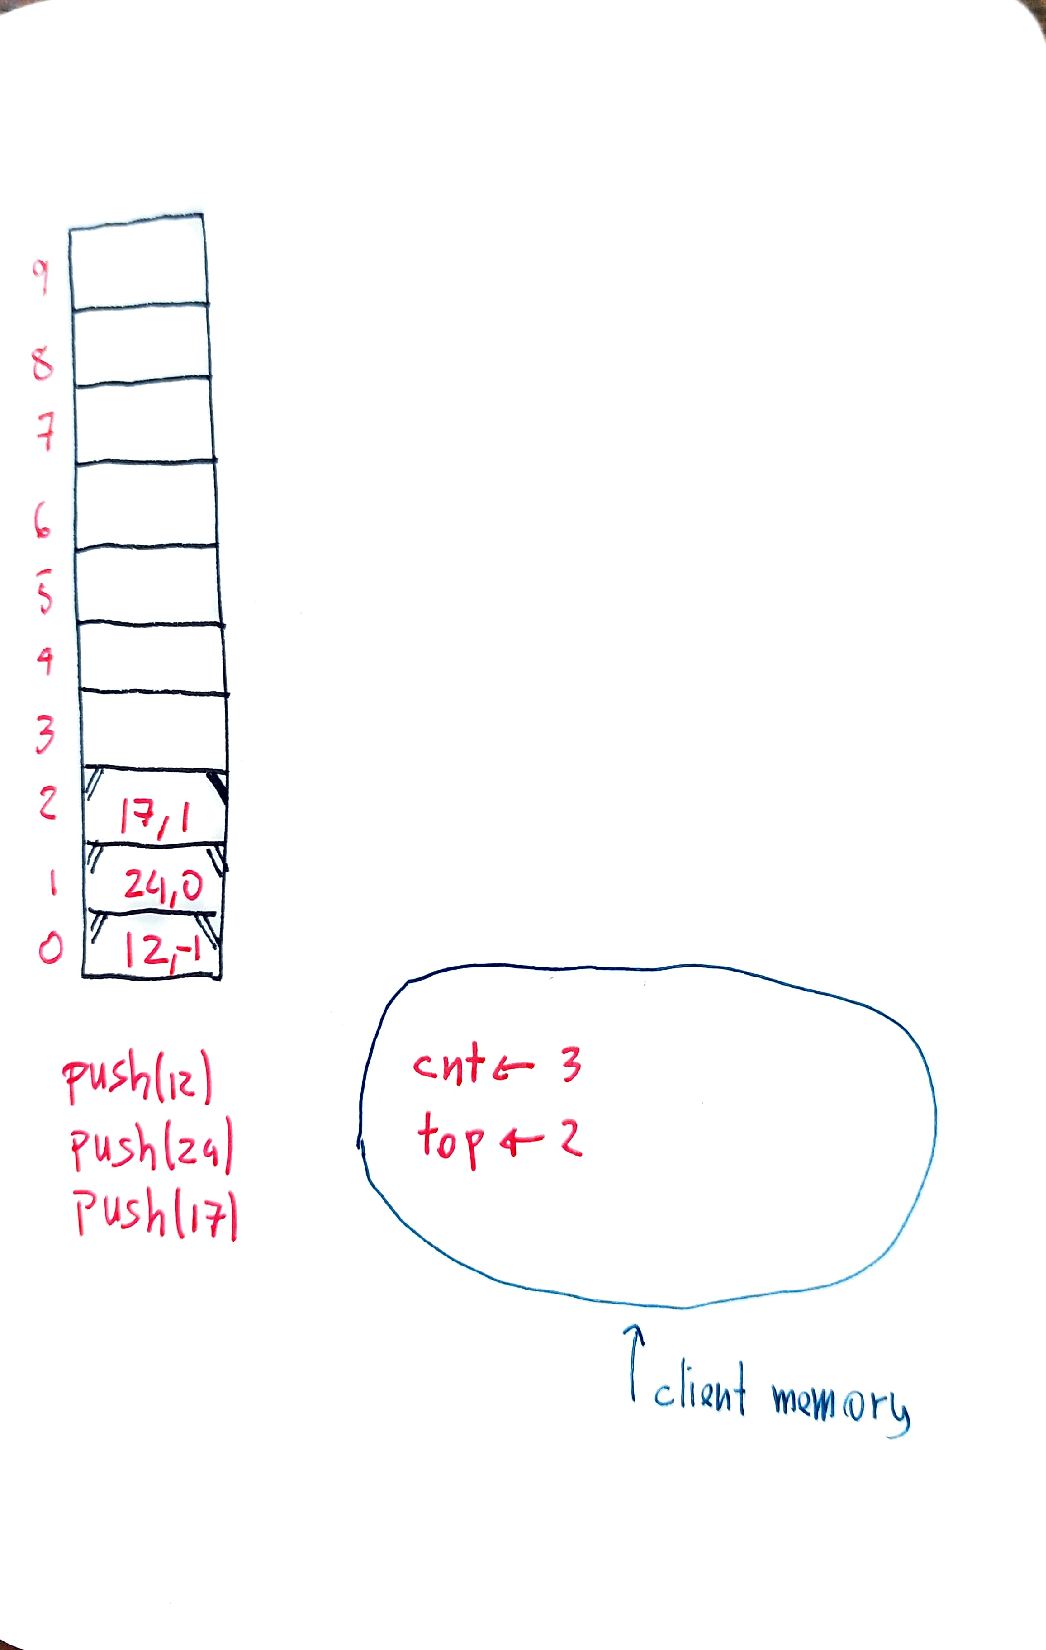
\includegraphics[height=9cm]{Images/stack-02.pdf}}
\only<3>{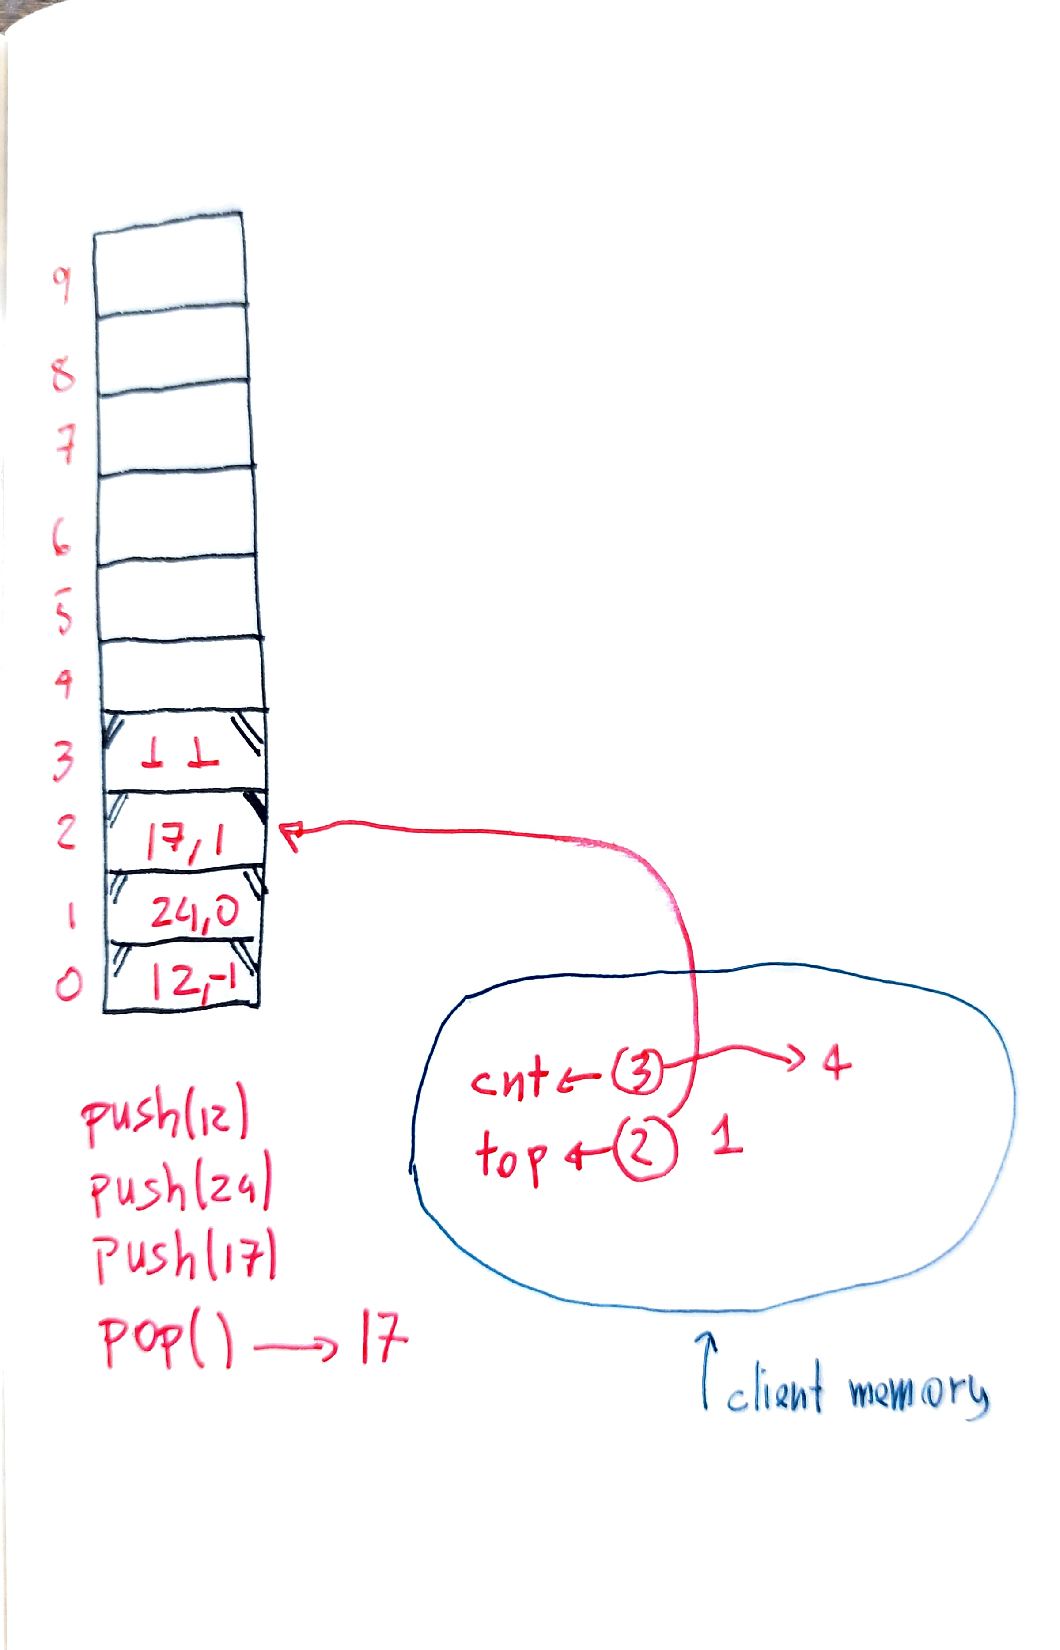
\includegraphics[height=9cm]{Images/stack-03A.pdf}}
\end{center}
\end{frame}

\begin{frame}
\begin{block}{Snapshot Secure Stacks}
\begin{itemize}
\color{blue}
    \item $\color{brown}\init()$
    \begin{itemize}
        \item randomly choose encryption key $\color{magenta}K$
        \item set $\color{magenta}\cnt=0$ and $\color{magenta}\tpp=-1$. 
    \end{itemize}
    \item $\color{brown}\push(v)$
    \begin{itemize}
        \item upload $\color{magenta}\enc(K,(v,\tpp))$ to location $\color{magenta}\cnt$
        \item set $\color{magenta}\tpp\leftarrow\cnt$
        \item set $\color{magenta}\cnt\leftarrow\cnt+1$
    \end{itemize}
    \item $\color{brown}\pop()$
    \begin{itemize}
        \item download pair $\color{magenta} (v,t)$
            from location $\color{magenta}\tpp$
        \item upload a dummy encryption to location
                $\color{magenta}\cnt$
        \item set $\color{magenta} \tpp\leftarrow t$ 
        \item set $\color{magenta}\cnt\leftarrow\cnt+1$
        \item return $\color{magenta} v$
  \end{itemize}
        
\end{itemize}
\end{block}
\end{frame}
    
\begin{frame}
\frametitle{Snapshot Security}

{\color{magenta} Snapshots: }

{\em \color{blue}
Only difference between operation $\color{teal} i$ and operation $\color{teal} i+1$ 
in location $\color{teal} i$
}

\pause
\vskip .1cm
{\em
{\color{teal} independent} {\color{blue} from history of ops}
}

\pause
\vskip 1cm 

{\color{magenta} Transcripts: }

{\em \color{blue}
Client reaches for the current {\color{teal} \tt top}
}

\pause
\vskip .2cm
{\em \color{blue}
Gives information about number of {\color{teal} \tt push} ops vs number of 
{\color{teal} pop} ops
}

\pause
\vskip 1cm 
{\em\color{brown}

    randomly select a {\color{teal} PRP} $\color{magenta} F$ and write new pair at 
$\color{magenta} F(\mathtt{cnt})$
}

\end{frame}
    
\begin{frame}
\frametitle{$(\infty,1)$-snapshot secure stacks}

$\color{purple}\calA$ gets snapshots of memory after 
{\color{teal} every operations} and transcript for {\color{teal} one}.

\pause


\begin{block}{Snapshot Secure Stacks}
\begin{itemize}
\color{blue}
    \item $\color{brown}\init()$
    \begin{itemize}
        \item randomly choose seed $\color{magenta}S$
        \item randomly choose encryption key $\color{magenta}K$
        \item set $\color{magenta}\cnt=0$ and $\color{magenta}\tpp=-1$. 
    \end{itemize}
    \item $\color{brown}\push(v)$
    \begin{itemize}
        \item download from location $\color{magenta}F(S,\tpp)$ and discard 
        \item upload $\color{magenta}\enc(K,(v,\tpp))$ to location $\color{magenta}F(S,\cnt)$
        \item $\color{magenta}\tpp\leftarrow\cnt$
        \item $\color{magenta}\cnt\leftarrow\cnt+1$
    \end{itemize}
    \item $\color{brown}\pop()$
    \begin{itemize}
        \item download pair $\color{magenta} (v,t)$
            from location $\color{magenta}F(S,\tpp)$
        \item upload dummy encryption at location 
            $\color{magenta}F(S,\cnt)$
        \item set $\color{magenta} \tpp\leftarrow t$ 
        \item set $\color{magenta}\cnt\leftarrow\cnt+1$
        \item return $\color{magenta} v$
  \end{itemize}
\end{itemize}
\end{block}
\end{frame}
    
\begin{frame}
\frametitle{This looks very promising}

\begin{itemize}
\item {\color{teal} Constant} slowdown against {\em\color{blue} snapshot} adversary
\begin{itemize}
    \item {\em for the same price I can throw in one transcript of your choice}
\end{itemize}
\item For {\em\color{blue} persistent} adversaries, stack is {\color{teal} as hard as ORAM}
\begin{itemize}
    \item Oblivious stack requires
       $$\color{magenta}\Omega(b/w) log(nb/c)$$
{\color{green} Riko Jacob, Kasper Green Larsen, Jesper Buus Nielsen. SODA 2019.}
\end{itemize}
\pause
\vfill
\item Actually, not! for ORAM is still 
       $$\color{magenta}\Omega(b/w) log(nb/c)$$
\pause

\vskip 1cm
{\color{red}\bf Sorry}
\end{itemize}
\end{frame}


\begin{frame}
\frametitle{The snapshot adversary}

\begin{block}{Snapshot window $(t,\ell)$}

\begin{itemize}
\item A {\em\color{blue} snapshot window} of length $\color{brown}\ell$ starting at time $\color{brown}t$.
\item The adversary receives
    \begin{itemize}
        \item {\color{magenta} snapshot} of server {\color{magenta} memory content}
            before operation $\color{brown}t$ has been executed
        \item {\color{magenta} transcript} of {\color{magenta} server's operations} for the following
            $\color{brown}\ell$ operations that take place at times 
            $\color{brown} t,t+1,\ldots,t+\ell-1$.
    \end{itemize}
\item For $\color{brown}\ell=0$, only memory content before operation $\color{brown}t$.
\end{itemize}
\end{block}
\begin{block}{A $(S,L)$-snapshot adversary}
Specifies a sequence of {\em\color{blue} snaspshot windows}
$\color{brown}\calS=((t_1,\ell_1),\ldots,(t_s,\ell_s))$ such that 

\begin{itemize}
\item $\color{brown}s\leq S$, at most $\color{brown}S$ {\color{brown} windows}, 
    \begin{itemize}\item at most $\color{brown}S$ {\color{blue} snapshots}\end{itemize}
\item $\color{brown}\sum \ell_i\leq L$, for a total duration of at most $\color{brown}L$ operations
    \begin{itemize}\item at most $\color{brown}L$ {\color{blue} transcripts}\end{itemize}
\end{itemize}
\end{block}
\end{frame}

\begin{frame}
\frametitle{The Lower Bound}

\begin{theorem}
\label{thm:strong}
For any $0\le\epsilon\le 1/16$,
let $\ds$ be a
\only<1-4>{$(3,1,\epsilon)$-snapshot}\only<5>{$({\color{blue}3,1,}\epsilon)$-snapshot}\only<6->{$(3,1,{\color{blue}\epsilon})$-snapshot}
private RAM data structure for 
\only<1>{$n$}\only<2>{$\color{blue}n$}\only<3->{$n$}
entries each of 
\only<1>{$b$}\only<2>{$\color{blue}b$}\only<3->{$b$}
bits implemented over 
\only<1-2>{$w=\Omega(\log n)$}\only<3>{$\color{blue}w=\Omega(\log n)$}\only<4->{$w=\Omega(\log n)$}
bits using client storage of 
\only<1-3>{$c$}\only<4>{$\color{blue}c$}\only<5->{$c$}
bits in the cell probe model.
If $\ds$ has amortized write time $t_w$ and expected amortized read time $t_r$ with failure probability at most 
$1/3$, then
$$
\color{blue} t_r+t_w = \Omega\left(b/w  \cdot \log(nb/c) \right).
$$
\end{theorem}
\only<2>{$\color{magenta} n$ {\em\color{brown}logical} blocks of $\color{magenta} b$ bits}
\only<3>{$\color{magenta}w<b$ is size {\em\color{brown}physical} words}
\only<4>{Client has $\color{magenta}c$ bits of {\em\color{brown}local memory}}
\only<5>{Adversary receives at most $\color{magenta}3$ memory {\em\color{brown} snapshots} and $\color{magenta}1$ operation {\em\color{brown} transcript}}
\only<6>{$\color{magenta}\epsilon$ is the adversary's advantage in the security game}
\end{frame}

\begin{frame}
\frametitle{The security game}

\begin{tcolorbox}
\noindent{$\color{magenta}{\mathbf \expt_{\ds,\calA}^{n,\beta}}$}
\begin{itemize}
\color{teal}
    \item Receive $\color{brown}(O_0,O_1,((t_1,\ell_1),\ldots,(t_{s},\ell_{s})))$ from $\color{purple} \calA_0(1^n)$.
    \item Set $\color{brown}\calL\leftarrow\emptyset$, $\color{brown}\ds\leftarrow(R_1,\ldots,R_n)$, $\color{brown}i \leftarrow 1$.
    \item While $\color{brown}i\le|O_\beta|$:
    \begin{itemize}
\color{teal}
        \item If $\color{brown}i = t_j$ for some $1\leq j\leq s$:
        \begin{itemize}
\color{teal}
            \item Set $\color{brown}\calL \leftarrow \calL \mid\mid (\mem, M)$.
            \item For $\color{brown}k=1,\ldots,\ell_j$:

                \quad Execute $\color{brown}\ds^{\mrl,\mwl}(O_b[i])$ and set $\color{brown}i \leftarrow i + 1$.
        \end{itemize}
        \item Else:

            \quad Execute $\color{brown}\ds^{\mr,\mw}(O_b[i])$ and set $\color{brown}i \leftarrow i + 1$.
    \end{itemize}
    \item Return $\color{purple}\calA_1(\calL)$.
\end{itemize}
\end{tcolorbox}
$$
\color{blue}\left|\Pr[\expt_{\ds,\calA}^{n,0}=1] - \Pr[\expt_{\ds,\calA}^{n,1}=1]\right| \le \epsilon,
$$
for all PPT $\color{purple}\calA$ that are $\color{magenta}(S,L)$-snapshot adversaries.
\end{frame}

\begin{frame}
\frametitle{The Epoch structure}

\begin{block}{The sequence and the epochs}
\begin{itemize}
\item $\color{magenta} n$ {\em logical indices}
\item $\color{magenta} m\leftarrow\{n/2+1,\ldots, n\}$
\item $\color{magenta} m$ writes of {\bf random} $\color{magenta} b$-bit blocks at indices
$\color{magenta}1,2,\ldots,m$
\item followed by {\color{magenta} one} read.
\end{itemize}
\end{block}


\vfill

\begin{center}
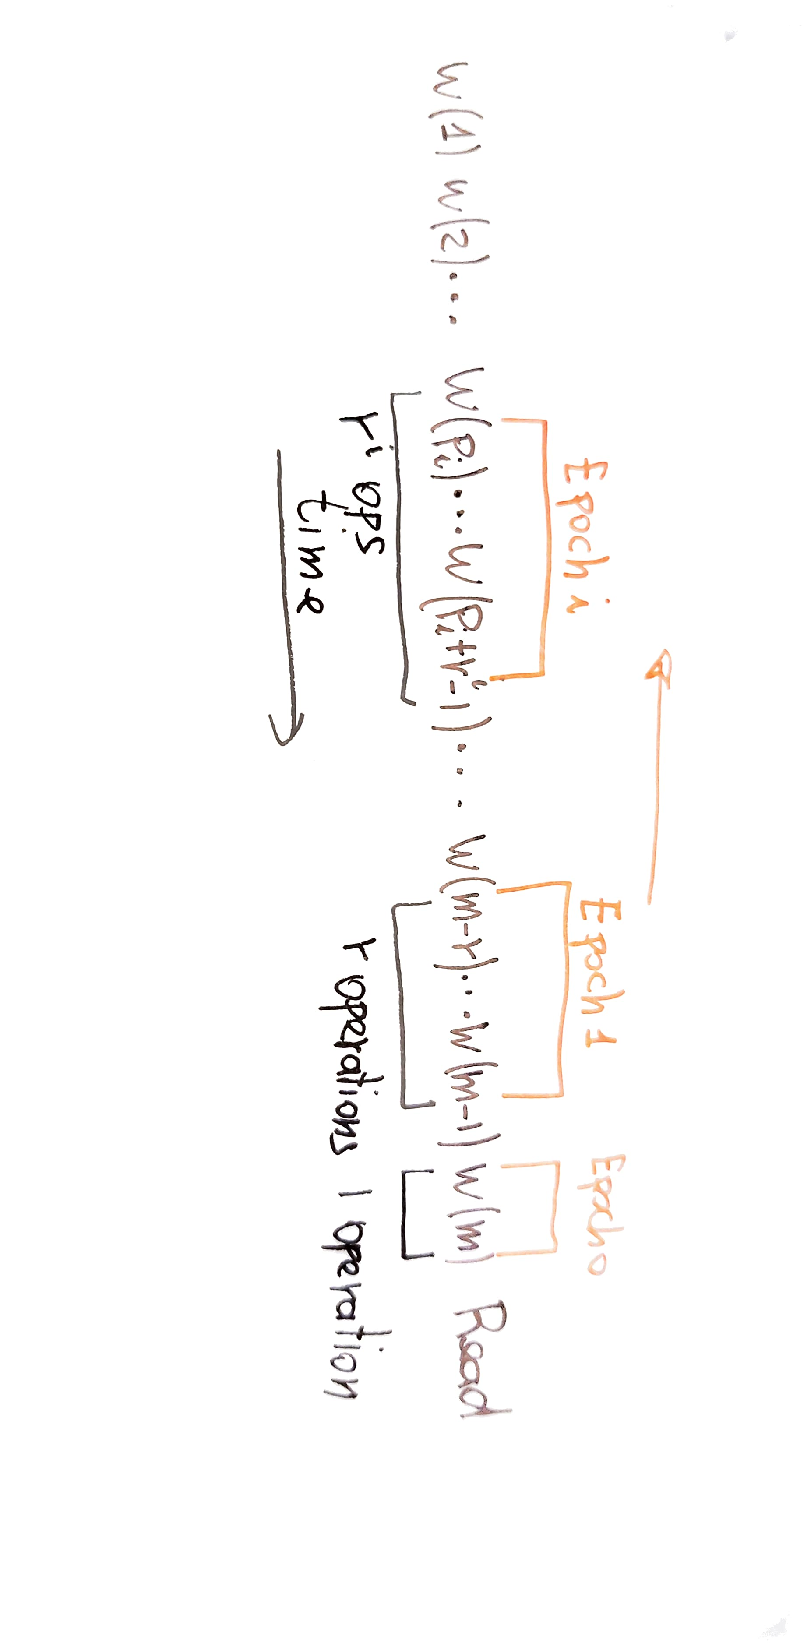
\includegraphics[angle=90,width=\textwidth]{Images/epochs.pdf}
\end{center}

\end{frame}

\begin{frame}
\frametitle{A $(3,1)$-snapshot adversary -- Intuition}

\begin{itemize}[<+->]
\color{teal}
\item Two sequences of operations $\color{brown} O_0, O_1$
\begin{itemize}
    \color{teal}
    \item Both write {\bf random} blocks to the first $\color{brown} m$ 
        indices
    \item $\color{brown} O_0$ reads index $\color{brown}{1}$
    \item $\color{brown} O_1$ reads a randomly selected index 
            $\color{brown} j$
            written in the $\color{brown}\mathbf{i}$-th epoch
\end{itemize}
\item {\bf correctness of $\color{brown} {O_1}$} 

    touch about $\color{brown} b/w$ cells updated
        in epoch $\color{brown} i$
\begin{itemize}
        \color{teal}
    \item epochs preceding epoch $i$ are {\bf independent}
    \item epochs following epoch $i$ are {\bf not large enough}
    \item pick $i$ so that client memory is {\bf too small}
\end{itemize}
\item {\bf correctness of $\color{brown} {O_0}$} 

    read of $\color{brown} O_0$ does not depend on epoch $\color{brown} i$

\item {\bf security}

    but if it does not, then security fails

\item{\bf final step} 

    this holds for {\em all} epochs except for those that have fewer
    than $c/b$ writes.

\item \color{magenta}\bf we have a lower bound
$\color{blue}\Omega(b/w\cdot\log(nb/c))$
\end{itemize}


\end{frame}

\begin{frame}
\frametitle{A $(3,1)$-snapshot adversary -- Part 0}

\begin{block}{$\calA_0^i(1^n)$}
\begin{itemize}
\color{teal}
   \item Randomly select integer $\color{brown}m$ from $\color{brown}[n/2,n]$.
   \item Randomly and ind. select $\color{brown}\bB_1,\ldots,\bB_m\from\zu^b$.
        \only<5>{\hfill{\color{purple} \bf Important}}
   \item Set $\color{brown}O_0=(\wri(1,\bB_1),\ldots,\wri(m,\bB_m),\re(m))$.
   \item Randomly select $\color{brown}j\in [p_i,p_i + r^i - 1]$,
   \item Set $\color{brown}O_1=(\wri(1,\bB_1),\ldots,\wri(m,\bB_m),\re(j))$.
   \item Set $\color{brown}\calS=((p_i,0),(p_i+r^i,0),(m+1,1))$.
   \item Return $\color{brown}(O_0,O_1,S)$.
\end{itemize}
\end{block}
\pause

\begin{itemize}[<+->]
\item $\color{brown}(p_i,0)$: 
{\color{magenta} snapshot} of server memory before epoch $i$ 
\item $\color{brown}(p_i+r^i,0)$: 
{\color{magenta} snapshot} of server memory after epoch $i$ 
\item $\color{brown}(m+1,1)$: 
{\color{magenta} snapshot} before read and {\color{magenta} transcript}  of read operation
\end{itemize}
\end{frame}

\begin{frame}
\frametitle{A $(3,1)$-snapshot adversary -- Part 1}

\begin{itemize}
\item $\color{magenta} U_i$ memory locations 
                overwritten during epoch $i$
    \begin{itemize}
        \item by comparing the {\color{brown} \bf initial}
        and {\color{brown}\bf final} snapshot of epoch $i$
    \end{itemize}
\item $\color{magenta} V_i$ memory locations overwritten since epoch $i$
    \begin{itemize}
        \item by comparing the {\color{brown}\bf final} snapshot of epoch $i$ 
    with snapshot {\color{brown} \bf before the read}
    \end{itemize}
\item $\color{magenta} W_i$ memory location overwritten during epoch $i$
that have not been modified when the read starts
    \begin{itemize}
        \item $\color{magenta} W_i=U_i\setminus V_i$
    \end{itemize}
\item $\color{magenta}Q_j$  cells from $\color{magenta}W_i$ read during
$\color{brown}\mathsf{read}(j)$, 
\item $\color{magenta} |Q_j|\approx b/w$ 
    \begin{itemize}
        \item $\color{purple}\calA^1$ returns 0 iff 
            $\color{magenta} |Q_j|\leq \rho\cdot b/w$ 
    \end{itemize}
\end{itemize}
\end{frame}

\begin{frame}
\frametitle{The coding argument}

\color{blue}
Suppose 
$$\color{magenta} t_w=o(b/w\log (nb/c))$$
then there exists $\color{magenta}\rho>0$ such that, for most 
epochs $\color{magenta}i$,
$$\color{magenta} |Q_j|\geq \rho\cdot b/w$$
with probability $\color{magenta}\geq 1/8$ for $\color{magenta} j$ in epoch 
$\color{magenta}i$. 

\pause

\vfill
{\bf Suppose not.}

\pause

Then we can encode the $r^i\cdot b$ bits of epoch $i$ using fewer bits.

\end{frame}
\begin{frame}

\frametitle{The coding argument - I}

\vfill

\begin{block}{A coding game}
\begin{itemize}
\item $\Sender$ wants to send $\color{red} \bB^i$ to $\Receiver$
    \begin{itemize}
    \item the $r^i$ blocks from {\color{blue} epoch $i$}
    \end{itemize}
\vskip .3cm
\item $\Sender$ and $\Receiver$ share 
    \begin{itemize}
        \item $\color{red} \bB^{-i}$ (all except epoch $i$) 
        \item randomness $\color{red}\calR$ to execute DS.
    \end{itemize}
\end{itemize}
\end{block}

\vfill
\vfill

$$\color{blue} {\cal{H}}(\bB^i|\calR, \bB^{-i})=r^i\cdot b.$$

\end{frame}

\begin{frame}
\frametitle{The coding argument - II}
\begin{itemize}
\item $\Sender$ and $\Receiver$ execute all epochs $\color{blue} >i$
$$\color{blue}\wri(1,\bB_1),\ldots,\wri(p_i-1,\bB_{p_i-1})$$


\begin{center}
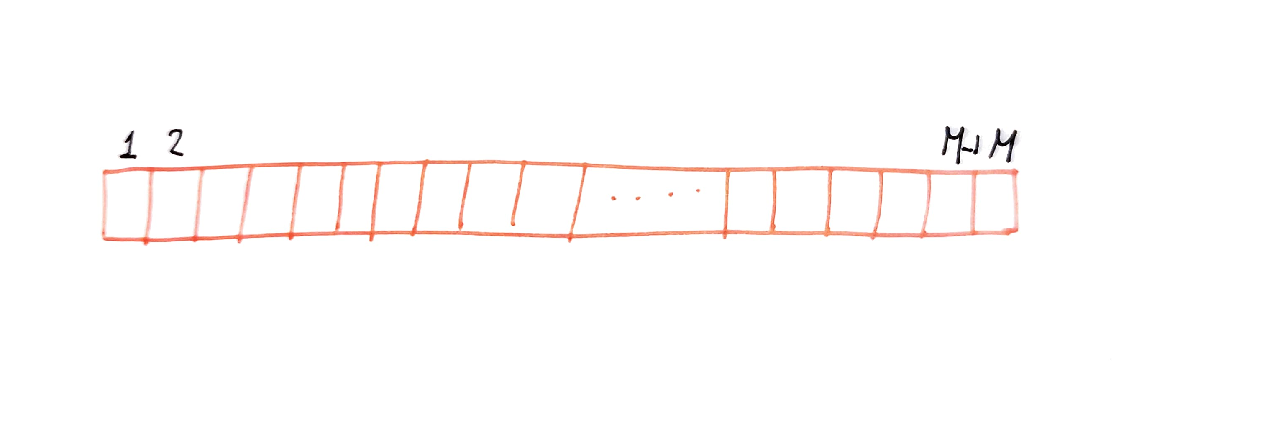
\includegraphics[width=\textwidth]{Images/memory01.pdf}
\end{center}
\end{itemize}
\end{frame}

\begin{frame}

\frametitle{The coding argument}
\begin{itemize}
\item $\Sender$ executes 
epoch $\color{blue}i$
$$\color{blue}\wri(p_i,\bB_{p_i}),\ldots,\wri(p_i+r^i-1,\bB_{p_i+r^i-1})$$
\item Note: $\Receiver$ cannot execute 
epoch $\color{blue}i$
\end{itemize}

\vfill

\begin{center}
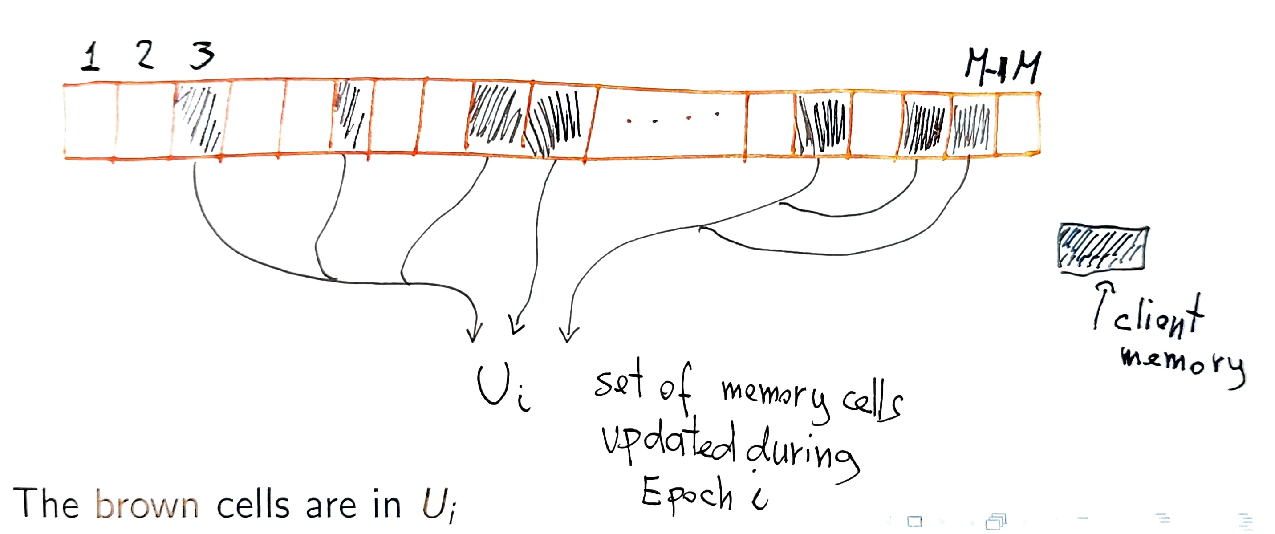
\includegraphics[width=\textwidth]{Images/memory02-A.pdf}
\end{center}

\end{frame}

\begin{frame}
\frametitle{The coding argument}
\begin{itemize}
\item $\Sender$ and $\Receiver$ execute epochs $\color{blue}<i$
    \begin{itemize}
        \item $\Receiver$ needs some help
    \begin{itemize}
        \item {\color{teal} client memory}: $\color{purple} c$ bits.
    \end{itemize}
    \end{itemize}
\vskip .3cm
\item For $\color{blue} j=p_{i-1},\ldots,m$
    \begin{itemize}
        \item execute $\color{blue}\wri(j,\bB_{j})$ touching $\color{blue} T_j$
        \item $\Receiver$ needs $\color{purple} U_i\cap T_j$ (cell location and content)
    \end{itemize}
\end{itemize}

{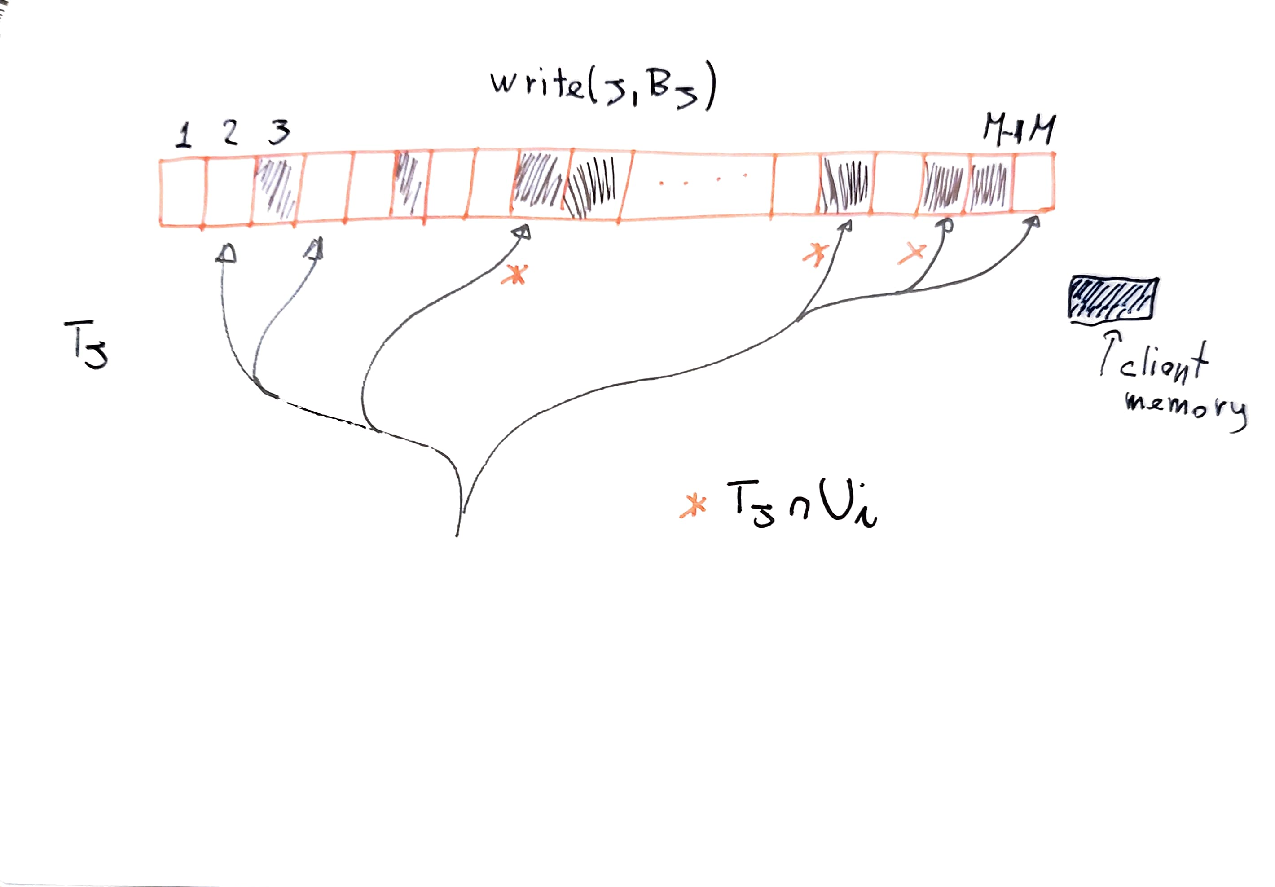
\includegraphics[width=\textwidth]{Images/memory04.pdf}}


\end{frame}

\begin{frame}
\frametitle{The coding argument}

\begin{itemize}
\item 
$\color{purple} c$ bits + set $\color{purple} Y_i:=U_i\cap (T_{p_i+r_i}\cup\cdots\cup T_m)$

\end{itemize}
{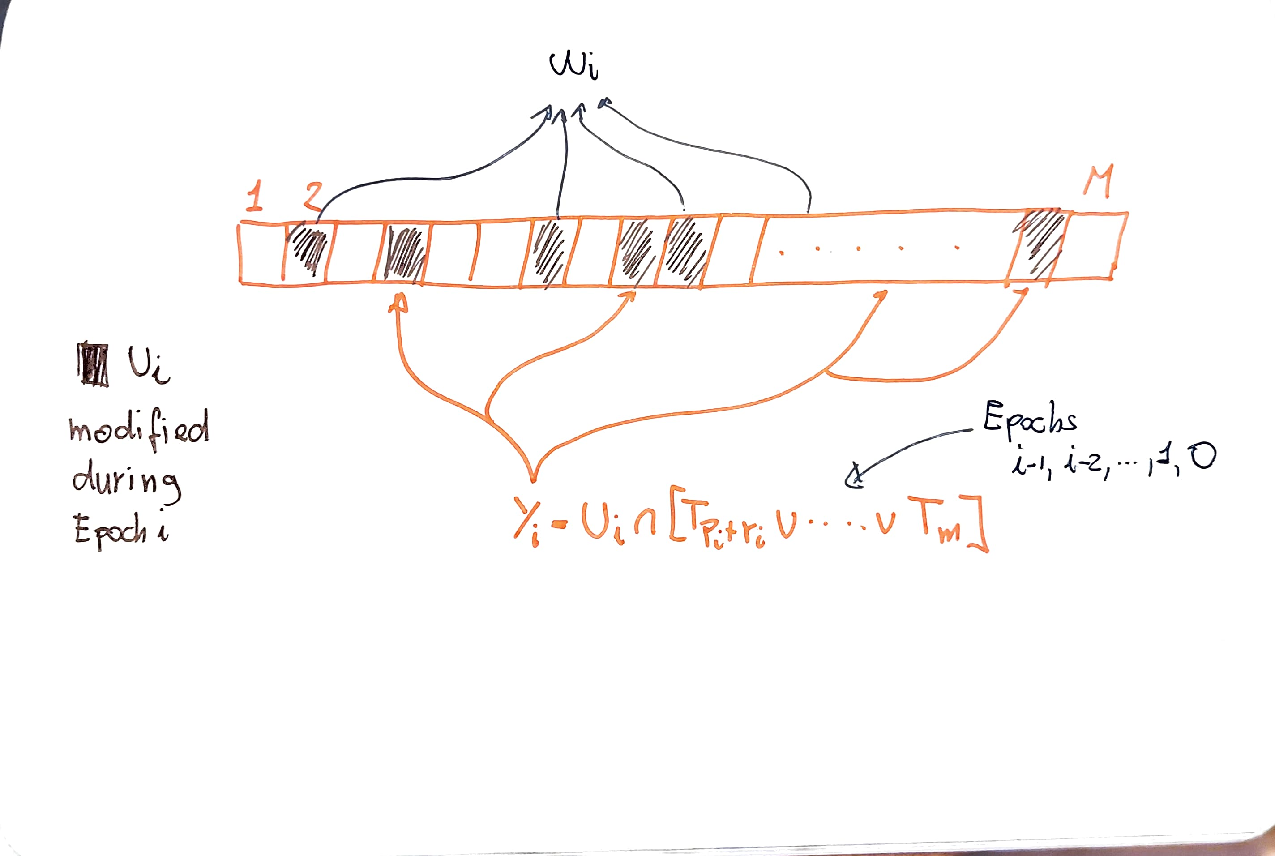
\includegraphics[width=\textwidth]{Images/memory05.pdf}}


\end{frame}

\begin{frame}
\frametitle{The coding argument}

$\color{teal}\mathbb{S}$ memory state after $\color{magenta}\wri(m,\bB_m)$
\vskip .3cm

\begin{itemize}
    \item For $\color{blue} j=p_i,\ldots,p_i+r^i-1$
    \begin{itemize}
        \item $\Sender$ and $\Receiver$ execute $\color{blue}\mathsf{read}(j)$ starting from 
        $\color{teal}\mathbb{S}$
        \item $\Receiver$ needs $\color{blue}Q_j:=W_i\cap T^{m}_j$
        \item if $\color{blue}\mathsf{read}$ errs or $\color{blue}Q_j>\rho b/w$
        \begin{itemize}
            \item $\color{blue} \bB_j$ is added to encoding
        \end{itemize}
        \item else
        \begin{itemize}
            \item $\color{blue} Q_j$ is added to encoding
        \end{itemize}

    \end{itemize}
\end{itemize}

\end{frame}

\begin{frame}

\frametitle{Length of encoding}


{\color{red}\bf Length depends on }
\vskip 1cm
\begin{itemize}
\item Set $\color{blue} Y_i$
    \begin{itemize}
        \item for most epochs $i$, 
            $\color{blue}\mathbb{E}[|Y_i|]\leq r^{i-1} b/w$
    \end{itemize}
\vskip .5cm
\item Set $\color{blue} Q_j$
    \begin{itemize}
        \item By assumption $\color{blue} |Q_j|<\rho\cdot b/w$ with prob $\color{blue} \geq 7/8$
    \end{itemize}
\end{itemize}

\pause
\vfill
\centerline{\bf\color{blue} Encoding is too small}
\end{frame}

\begin{frame}
\frametitle{Getting there...}
$$\color{magenta} t_w=o(b/w\log (nb/c))$$
implies that, for most epochs $\color{magenta}i$,

\only<1>{
$$\color{magenta} |Q_j|\geq \rho\cdot b/w$$
with probability $\color{magenta}\geq 1/8$ for $\color{magenta} j$ in epoch 
$\color{magenta}i$. 
}
\only<2->{\vskip 1cm
$\color{purple}\calA$ outputs $1$ with probability $\color{magenta}\geq 1/8$ when reading 
$\color{magenta} j$} from 
epoch $\color{magenta}i$. 

\only<3->{\vskip .4cm
If $\color{magenta}\epsilon=1/16$
    then $\color{purple}\calA$ outputs $1$ with probability $\color{magenta}\geq 1/16$ when reading 
$\color{magenta} m$}

\only<4->{\vskip .4cm
$\color{magenta} \mathsf{read}(m)$ must touch $\color{magenta} \geq \rho\cdot b/w$
cells from epoch $\color{magenta} i$
}

\only<5->{\vskip .4cm
$$\color{magenta} \Omega(b/w\cdot \log nb/c)$$
}
\end{frame}

\begin{frame}
\frametitle{Wrapping up}

\begin{block}{Now...}
If writes are fast
$$\color{magenta} t_w=o(b/w\log (nb/c))$$
then $\color{magenta}\mathsf{read}(j)$ in epoch $\color{magenta} i$ has
$\color{magenta} Q_j=\Omega(b/w)$
with prob at least $1/8$.
\end{block}

\pause

\begin{block}{Reading 1}
Must touch from each large epoch $\color{magenta}O(b/w)$ cells otherwise we lose security.

$$\color{magenta}\Omega(b/w\cdot \log(nb/c))$$
\end{block}
\end{frame}

\end{document}
